\documentclass[12pt,a4paper,final]{report}
\usepackage[cm]{fullpage}
\usepackage[utf8x]{inputenc}
\usepackage{listings}
\usepackage{color}
\usepackage{textcomp}
\usepackage{graphicx}
\usepackage{float}
\graphicspath{/home/thoorfr/NetBeansProjects/GeoImageViewer/doc/}
\usepackage[pdfborder={0 0 0 0}]{hyperref}
\restylefloat{figure} % to force position of figure
\newcommand{\HRule}{\rule{\linewidth}{0.5mm}}

\author{Francois-Xavier Thoorens}
\title{SUMO End-User Manual}

%%%%%%%%%%%%%%%%%%%%%%%%%%%%%%%%%%%%%%%%%%%%%%%%%%%%%%
%%%%%%%%%%%%%  DOCUMENT START HERE %%%%%%%%%%%%%%%%%%%
%%%%%%%%%%%%%%%%%%%%%%%%%%%%%%%%%%%%%%%%%%%%%%%%%%%%%%

\begin{document}
\begin{titlepage}
 
\begin{center}
 
 
\textsc{\LARGE EC-JRC-IPSC-MARITIME AFFAIRS-VESPO}\\[1.5cm]
 
\HRule \\[0.4cm]
{\huge \bfseries SUMO End-User Manual}\\[0.4cm]
\HRule \\[1.5cm]
 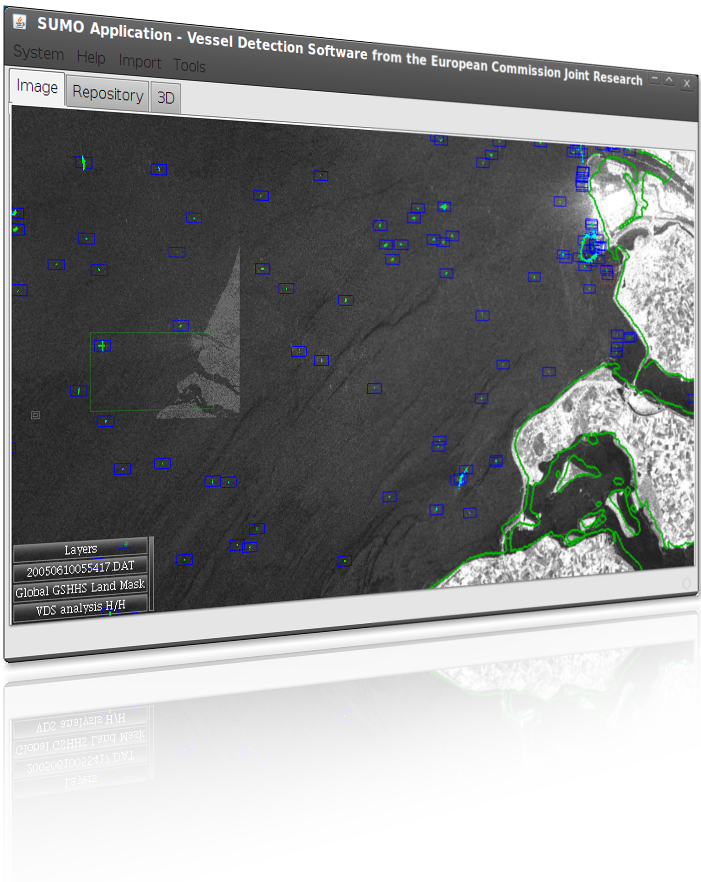
\includegraphics[scale=0.35,keepaspectratio=true]{./images/SUMO_reflection.png}\\[1cm]
\begin{minipage}{0.4\textwidth}
\begin{flushleft} \large
\emph{Author:}\\
Francois-Xavier \textsc{Thoorens}
\end{flushleft}
\end{minipage}
\begin{minipage}{0.4\textwidth}
\begin{flushright} \large
\emph{Version:} \\
\textsc{Draft}
\end{flushright}
\end{minipage}
 
\vfill

% Bottom of the page
{\large \today}
 
\end{center}
 
\end{titlepage}

\tableofcontents



\chapter{Introduction}
%%%%%%%%%%%%%%%%%%%%%%
\section{History}
\textbf{SUMO} stands for \textbf{S}earch for \textbf{U}nidentified \textbf{M}arine \textbf{O}bject.
It is a software originally dedicated to help researchers of the JRC to deal with SAR satellite images as well as a platform to help fisheries management staff to use remote sensing in the frame of FP research projects (IMPAST, DECLIMS, LIMES, TANGO) or other framework (MARISS).
This Software has been developed since 2003 and is first referenced by:

``Integrating Remote Sensing in Fisheries Control'', N. Kourti, I. Shepherd, H. Greidanus, M. Alvarez, E. Aresu, T. Bauna, J. Chesworth, G. lemoine, G. Schwarz, Fisheries management and Ecology vol. 12 p. 295-307, BLACKWELL PUBL LTD, 2005

More information at

\url{http://publications.jrc.ec.europa.eu/repository/handle/111111111/13106}

\section{General Description}
The \textbf{SUMO} interface is divided into three logics: 
\begin{enumerate}
 \item The Image View where the user interact to explore the loaded image.
 \item The World Wind view showing the earth to be able to locate the geolocation of the image.
 \item The Plugins part that are mostly situated in the menus
\end{enumerate}


\begin{figure}[H]
 \centering
 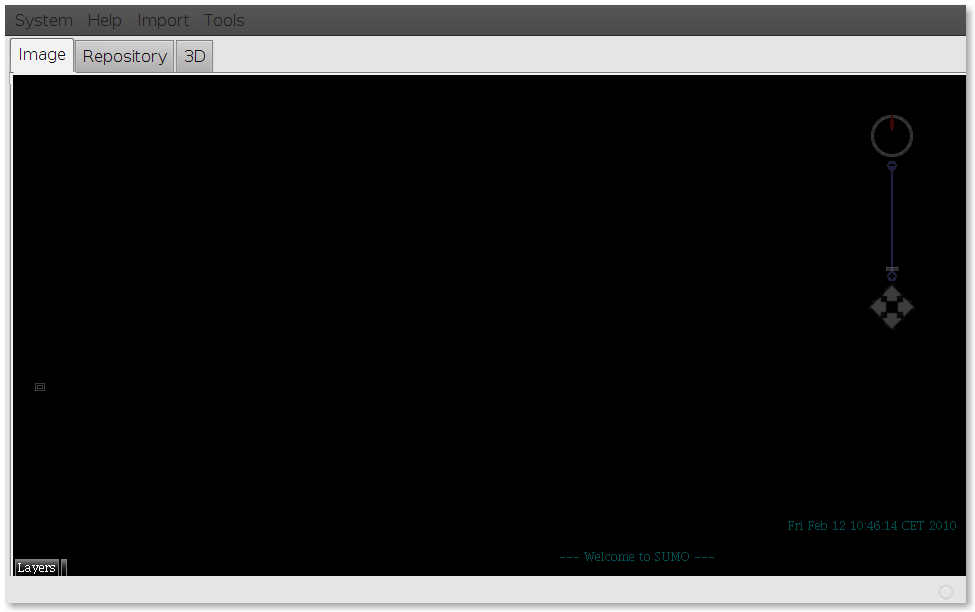
\includegraphics[scale=0.45,keepaspectratio=true]{./images/SUMOImageView.png}
 \caption{The SUMO Image View}
\end{figure}

\begin{figure}[H]
 \centering
 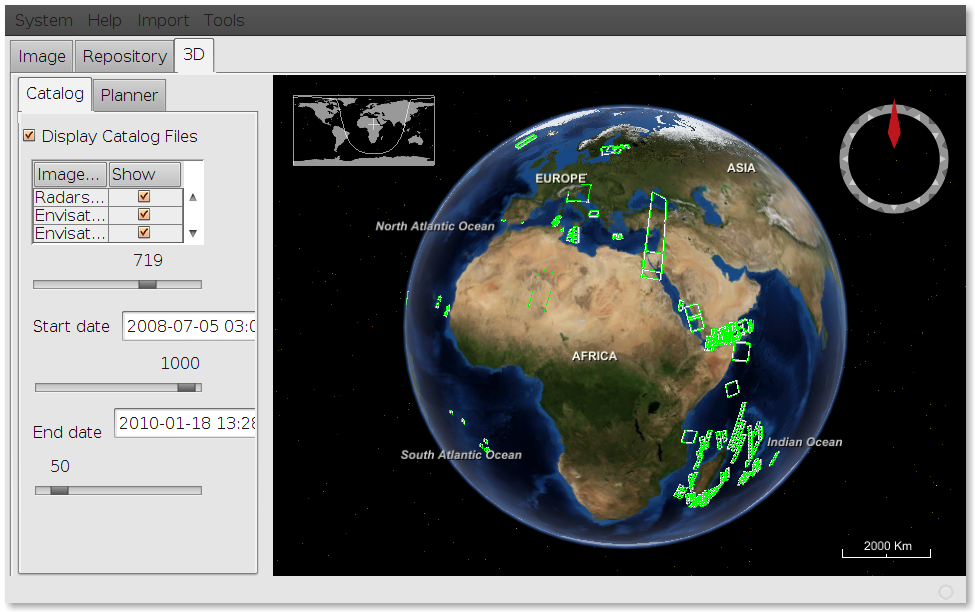
\includegraphics[scale=0.5,keepaspectratio=true]{./images/SUMOWWView.png}
 \caption{The SUMO WorldWind View}
\end{figure}

The manual is divided in Use Cases in order to refers quickly to the user needs, and also to quickly find out if what the user want to do is possible or not.

\chapter{Installation}
\section{Environment Requirements}
%---------------------------------%
\subsection{Minimum}
\begin{itemize}
\item RAM: 512K
\item CPU: 1GHz
\item Graphic Card: supporting OpenGL 2.0. Don't forget to update your drivers.
More information at \url{http://worldwind.arc.nasa.gov/java/video.html}
\end{itemize}
\subsection{Recommended}
\begin{itemize}
\item RAM: 2G
\item CPU: dual core 1.8 GHz
\item Graphic Card: NVidia GForce
\end{itemize}
You need to have the Java Virtual Machine (JRE) version $\geq$ 1.5 installed on your machine.
Check \url{http://java.sun.com} for more information.

\section{Starting Up The Application}
The application is a jar file with numerous dependencies.
You need to startup using the following command line:
\\
\texttt{\small{java -Xmx512m -Djava.library.classpath=. -Dsun.java2d.noddraw=true -jar GeoImageViewer.jar $>$ log.txt}}
\\
You can save this command line in a file called \textbf{startup.sh} (\textbf{startup.bat} for windows platform) and double click on it to start up the application.

Note that if you have enough RAM (i.e. minimum 2G) you can speed up the application setting -Xmx1024m instead of -Xmx512m.
It allocates 1G of RAM for the application instead of 512M.


\chapter{Use Cases}
\section{Opening an Image: Import $>$ Image}
\begin{figure}[H]
 \centering
 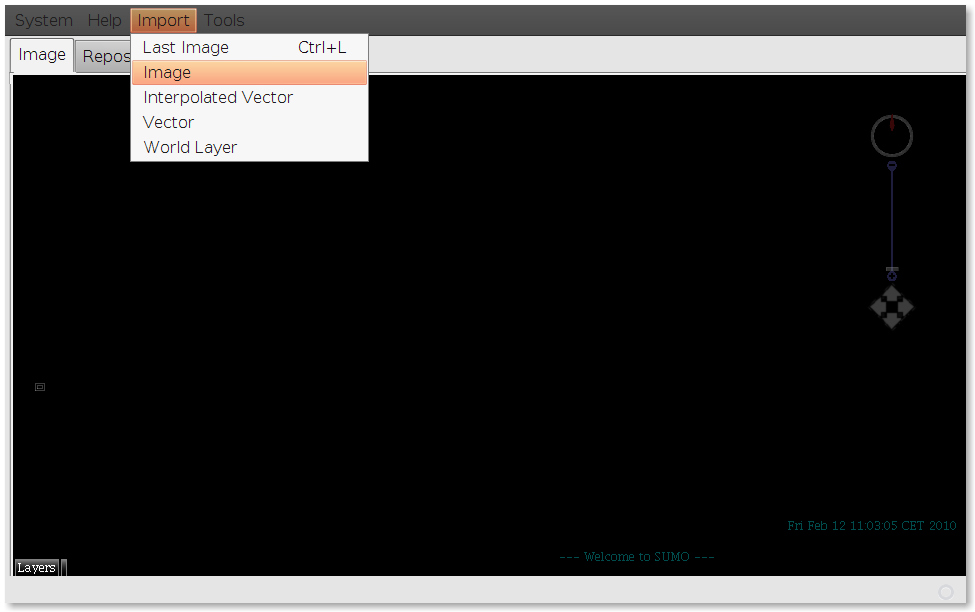
\includegraphics[scale=0.45,keepaspectratio=true]{./images/ImportImage.png}
 \caption{Open Image}
\end{figure}
\begin{figure}[H]
 \centering
 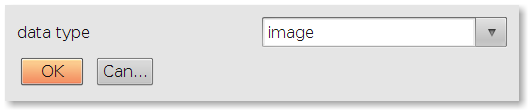
\includegraphics[scale=0.45,keepaspectratio=true]{./images/ImportImage2.png}
 \caption{Open Image}
\end{figure}
\begin{figure}[H]
 \centering
 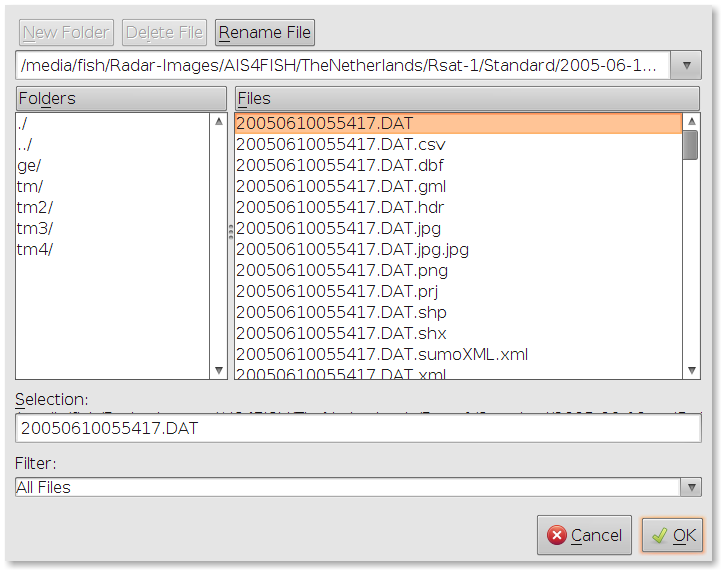
\includegraphics[scale=0.45,keepaspectratio=true]{./images/ImportImage3.png}
 \caption{Open Image}
\end{figure}
\begin{figure}[H]
 \centering
 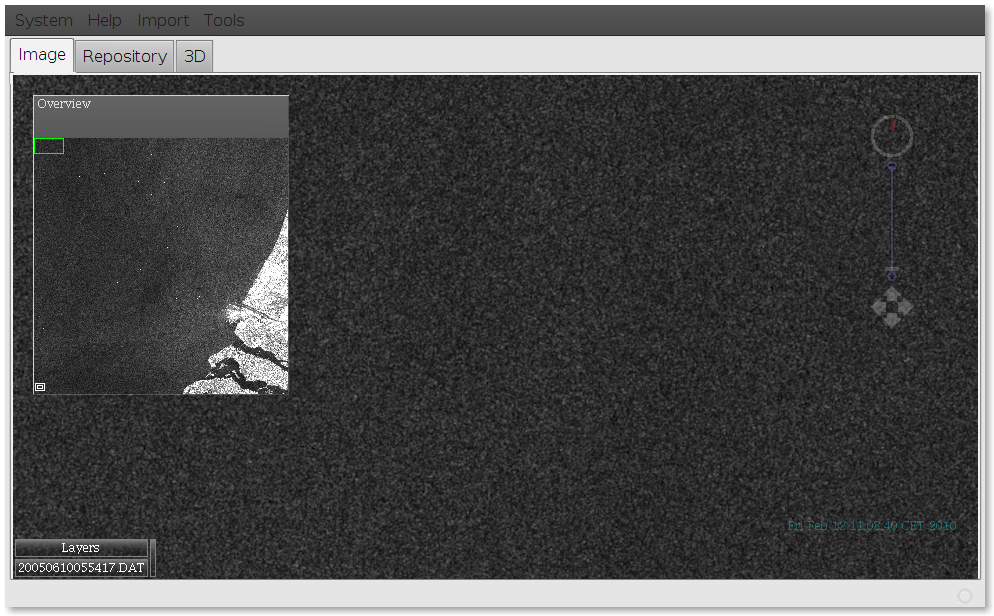
\includegraphics[scale=0.45,keepaspectratio=true]{./images/ImportImage4.png}
 \caption{Open Image}
\end{figure}

To open the last used image you can use \textbf{Import $>$ Last Image} or the shortcut \textbf{CTRL+L}.

\section{Adding Embedded Land Mask: Import $>$ World Layer}
\begin{figure}[H]
 \centering
 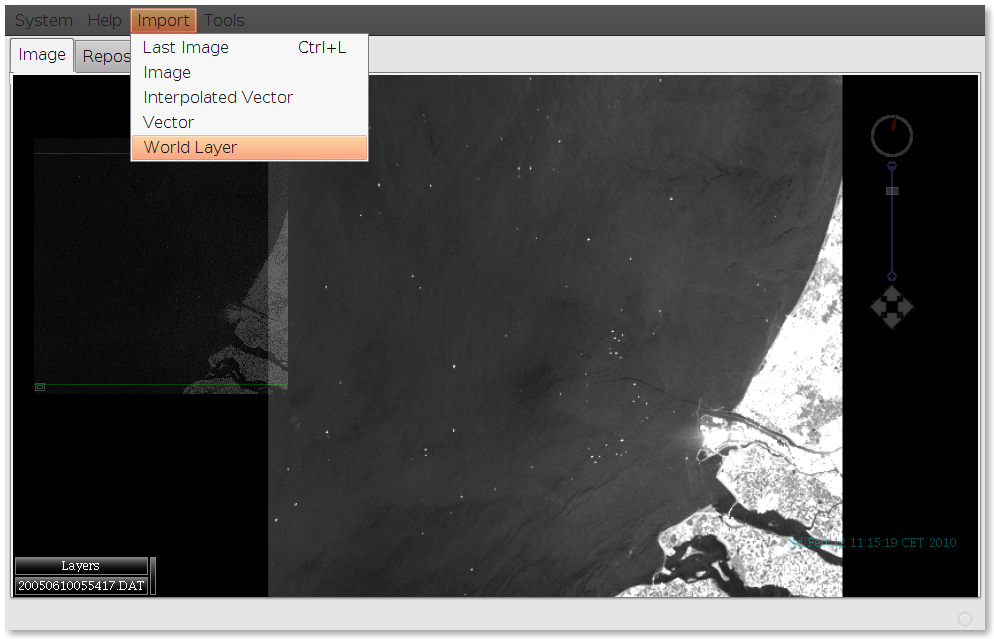
\includegraphics[scale=0.45,keepaspectratio=true]{./images/LandMask1.png}
 \caption{Add Land Mask}
\end{figure}
\begin{figure}[H]
 \centering
 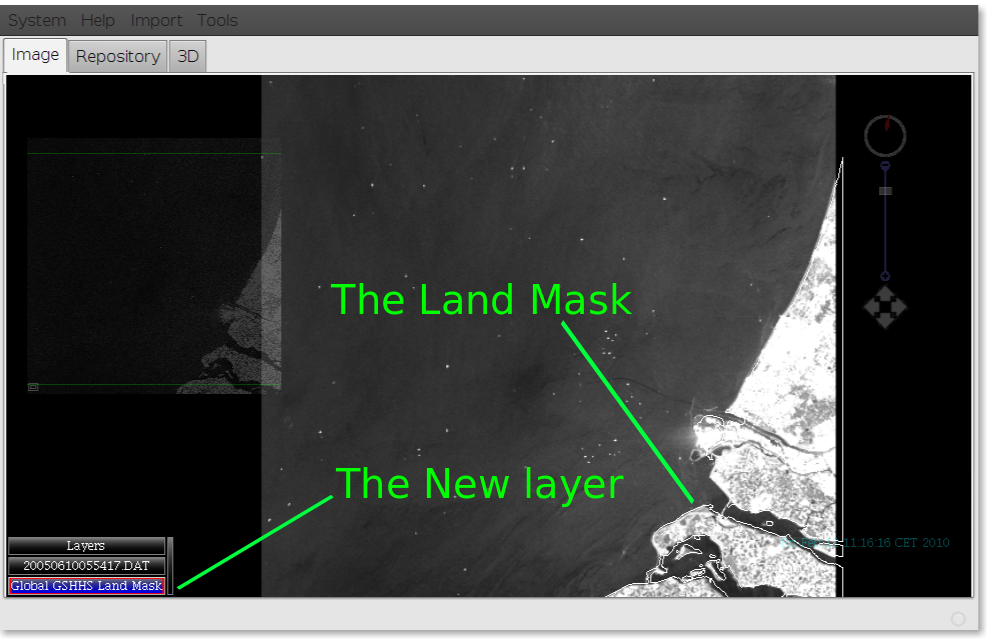
\includegraphics[scale=0.45,keepaspectratio=true]{./images/LandMask2.png}
 \caption{The land mask is added as 'Global GSHHS Land Mask'}
\end{figure}

\section{Navigating in the Image}
\subsection{With the Mouse}
Hold the \textbf{SHIFT} key and move the mouse around the center of the image, the general rules:
\begin{itemize}
 \item Get the mouse pointer far from the center of the view to accelerate the navigation
 \item The vector drawn by the the center point and the mouse pointer position indicates the movement of the navigation
 \item Stop moving the mouse pointer to stop the navigation
\end{itemize}
Use the Middle wheel to \textbf{Zoom In/Zoom Out}
\subsection{With the Overview Widget}
Click on the small square at the bottom left of the Overview widget to enable/disable interaction with it.
The green frame in the widget delimits the focused area and is updated as soon as you zoom In/Out or move the area of interest.
\begin{figure}[H]
 \centering
 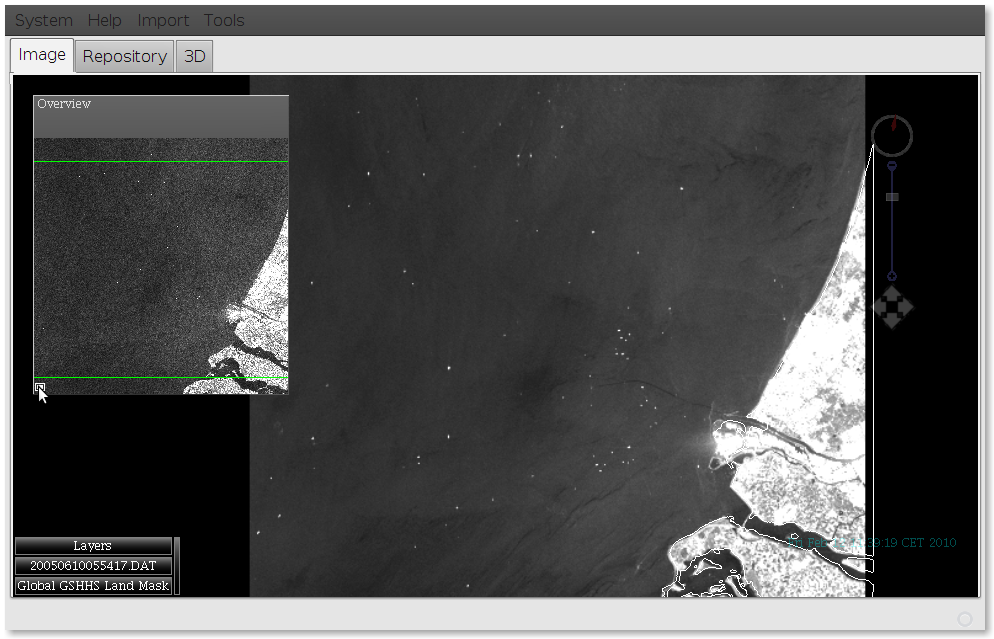
\includegraphics[scale=0.45,keepaspectratio=true]{./images/OverviewNavigation.png}
 \caption{The Overview Widget Disable/Enable}
\end{figure}

Once enabled, click on the overview to focus the area of interest, the image view is updated automatically.

\begin{figure}[H]
 \centering
 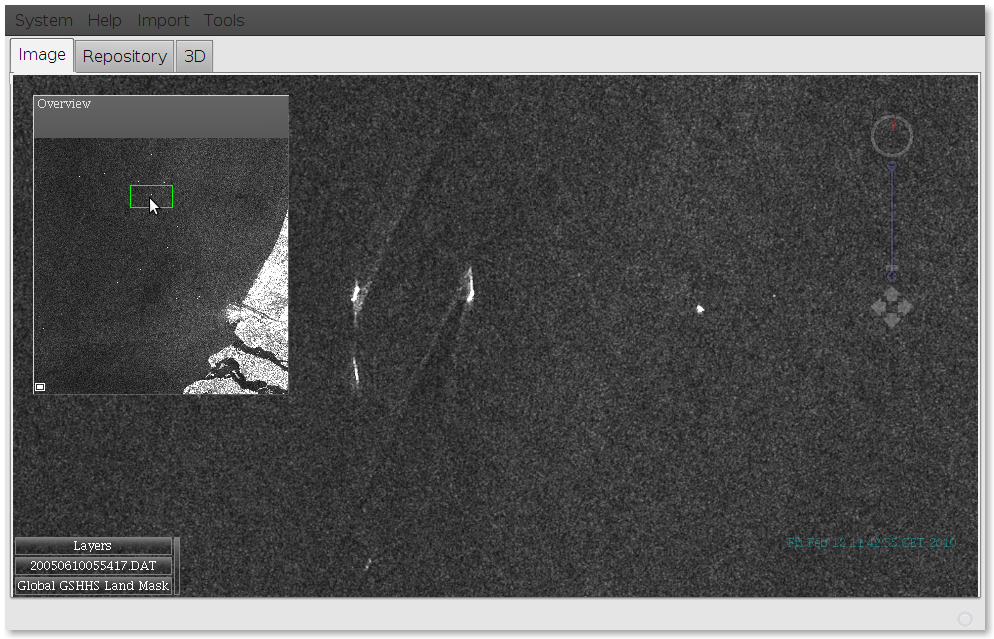
\includegraphics[scale=0.45,keepaspectratio=true]{./images/OverviewNavigation2.png}
 \caption{The Overview Widget Click \& Focus}
\end{figure}

\subsection{With the Keyboard}
  There are several keyboard  keys to navigate the image.
The view having the focus, the following commands can be used for navigation:
\begin{itemize}
 \item \textbf{Shift + \textuparrow}: move up
 \item \textbf{Shift + \textrightarrow}: move right
 \item \textbf{Shift + \textleftarrow}: move left
 \item \textbf{Shift + \textdownarrow}: move down
 \item type \textbf{``home'' + enter}: zoom out so you view the full image.
You may also use the shortcut \textbf{``h'' + enter}
\end{itemize}

\section{Inspecting Image Properties}
In order to open the properties window of the image \textbf{Right Click} on the image layer.
\begin{figure}[H]
 \centering
 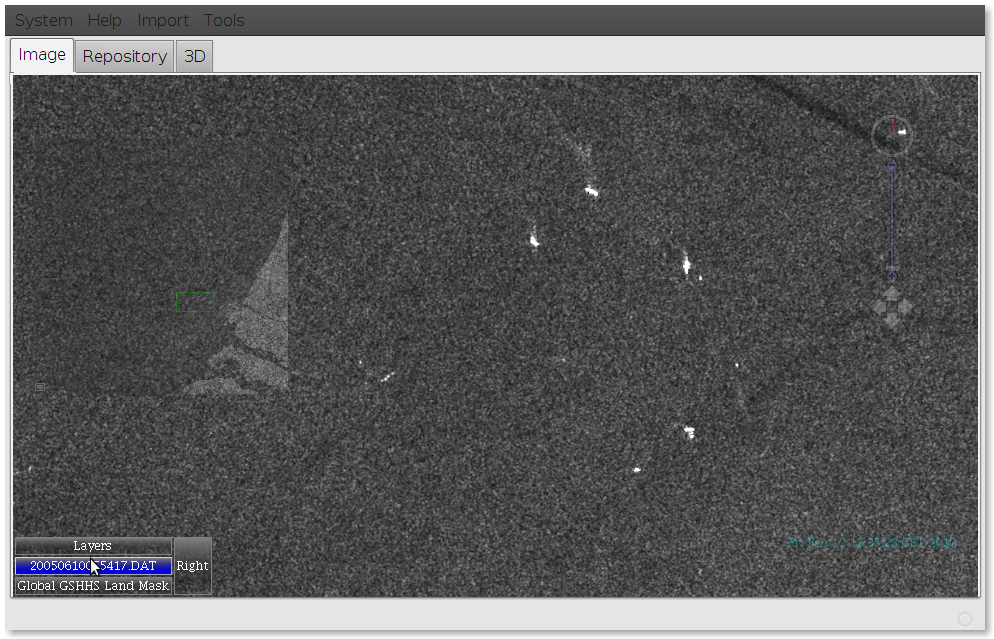
\includegraphics[scale=0.45,keepaspectratio=true]{./images/ImageProperties1.png}
 \caption{Right Click on the Image Layer}
\end{figure}
\begin{figure}[H]
 \centering
 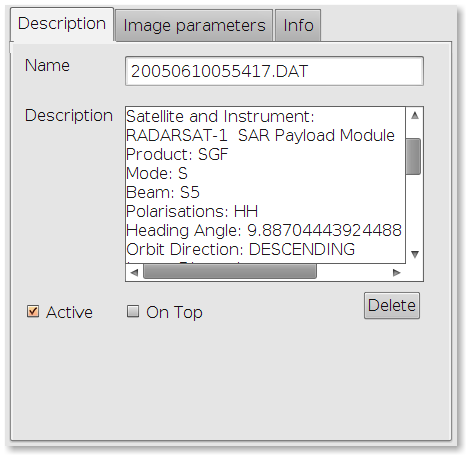
\includegraphics[scale=0.45,keepaspectratio=true]{./images/ImageProperties2.png}
 \caption{Description of the Image Metadata}
\end{figure}
\begin{figure}[H]
 \centering
 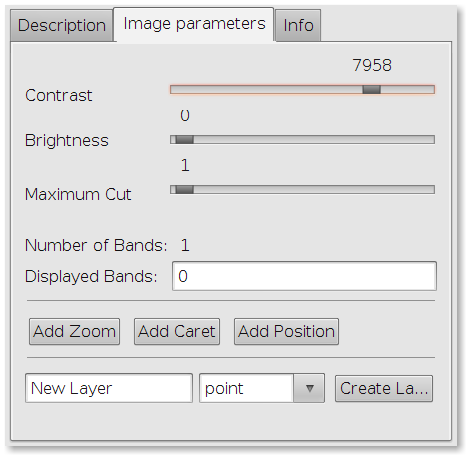
\includegraphics[scale=0.45,keepaspectratio=true]{./images/ImageProperties3.png}
 \caption{Changing Image Settings: contrast, brightness, displayed band}
\end{figure}

From the \textbf{Image Parameters} tab you can open three more layers:
\begin{itemize}
 \item \textbf{Add Zoom} will add the zoom associated with the current band (as shown in the \textbf{Displayed Bands} parameter).
If you need to put several bands in the zoom hit again the button \textbf{Add Zoom} with a different value in \textbf{Displayed Bands} parameters
\begin{figure}[H]
 \centering
 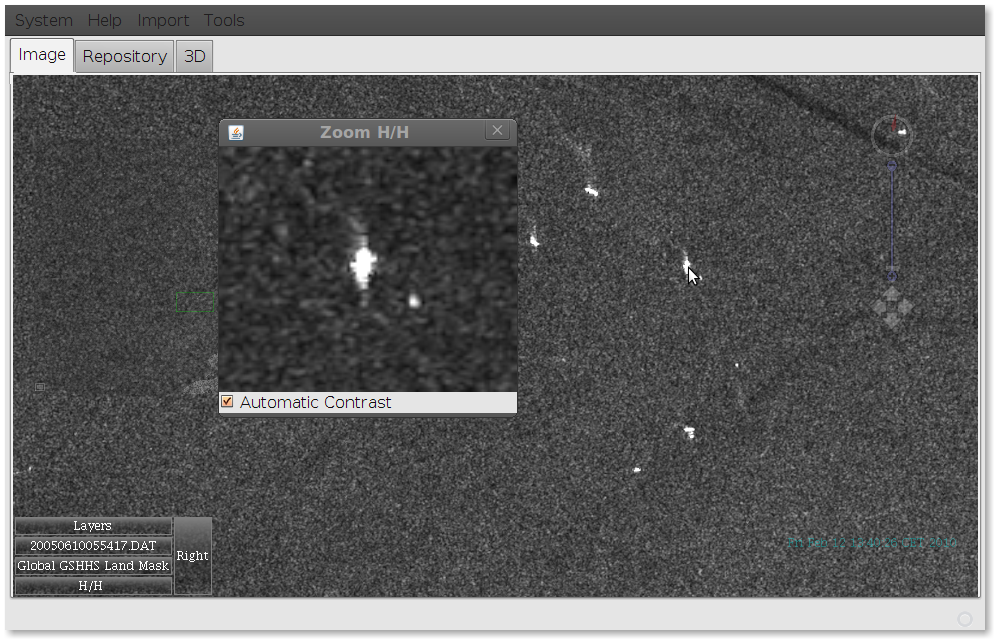
\includegraphics[scale=0.45,keepaspectratio=true]{./images/ZoomWindow.png}
 \caption{The use of Zoom windows. It displays the area under the pointer of the mouse}
\end{figure}

 \item \textbf{Add Caret} will add a caret showing the focused area.
The caret is equivalent to the green frame of the \textbf{Overview Widget} but is relative to the image view port
so it is slightly distorted if your application shows rectangular.
\begin{figure}[H]
 \centering
 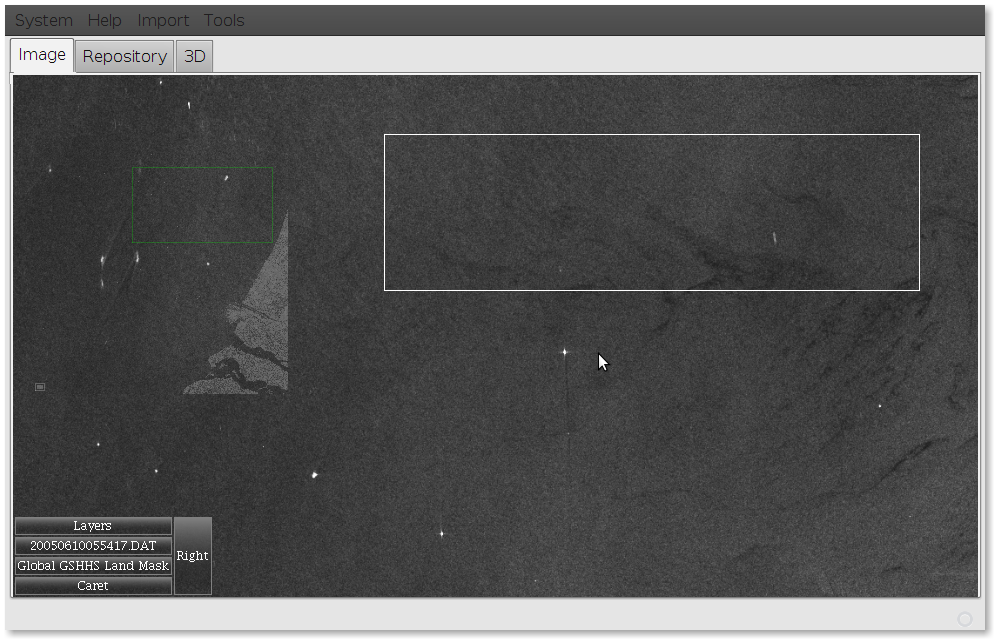
\includegraphics[scale=0.45,keepaspectratio=true]{./images/CaretLayer.png}
 \caption{The White frame is the Caret}
\end{figure}
 
 \item \textbf{Add Position} will pop up a window showing the current position of the pointer of the mouse in the image pixel reference as well as the geographic reference (default is \textbf{EPSG:4326}).
\begin{figure}[H]
 \centering
 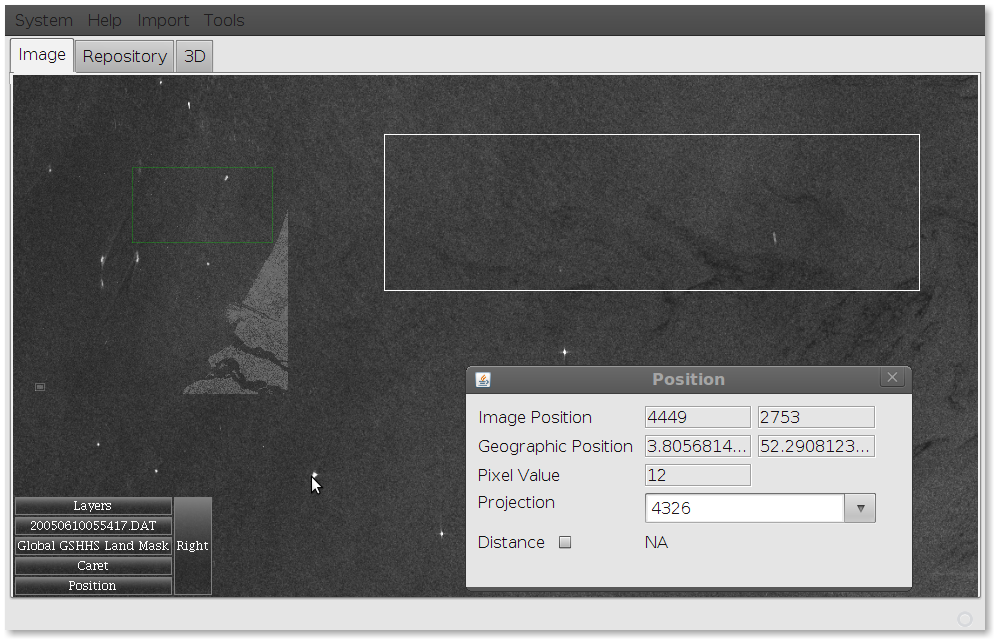
\includegraphics[scale=0.45,keepaspectratio=true]{./images/PositionLayer.png}
 \caption{The Position Window}
\end{figure}

\begin{figure}[H]
 \centering
 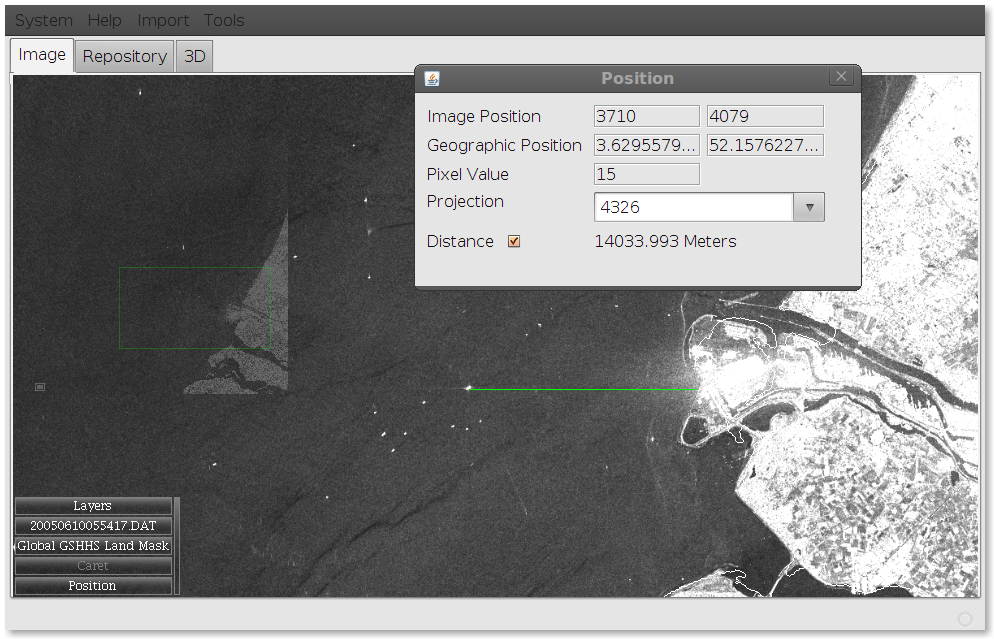
\includegraphics[scale=0.45,keepaspectratio=true]{./images/DistanceCalculation.png}
 \caption{Performing distance calculation in the Position window, in meters}
\end{figure}
 
\end{itemize}

\section{Performing a VDS Analysis: Tools $>$ VDS}
\begin{figure}[H]
 \centering
 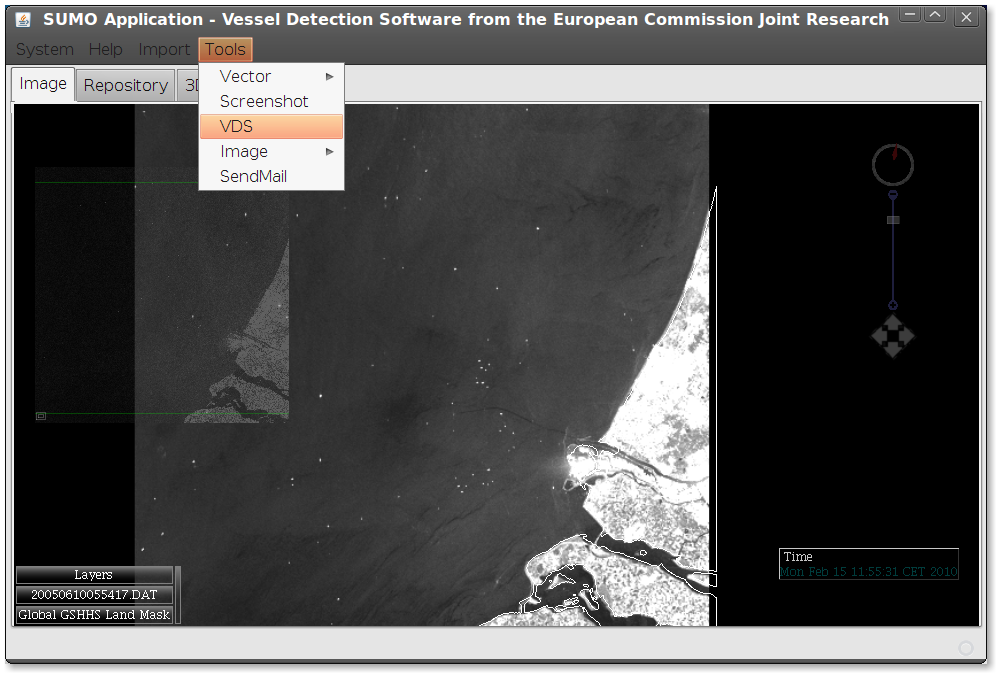
\includegraphics[scale=0.45,keepaspectratio=true]{./images/VDS1.png}
 \caption{Start the VDS tool}
\end{figure}

\begin{figure}[H]
 \centering
 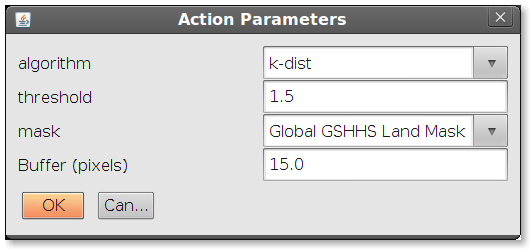
\includegraphics[scale=0.45,keepaspectratio=true]{./images/VDS2.png}
 \caption{Select parameters of the VDS analysis}
\end{figure}

The parameters needed for the VDS analysis are the following:
\begin{enumerate}
 \item \textbf{algorithm}: the algorithm used for the detection (\textbf{default}: k-dist)
 \item \textbf{threshold}: the value used to sort out  false alarms.
The higher the value, the more you discard targets based on their contrast from the background noise (\textbf{default}: 1.5)
 \item \textbf{mask}: the Vector Layer used for masking the land (optional) (\textbf{default}: the first loaded vector layer)
 \item \textbf{Buffer (pixels)}: the size of the buffer for the mask data.
A new vector data will be created and the original data will remain untouched. (\textbf{default}: 15) 
\end{enumerate}
When you press \textbf{OK} the analysis starts and covers all the available bands of the image.
It also performs a merged analysis gathering and merging the results of all the bands.

\begin{figure}[H]
 \centering
 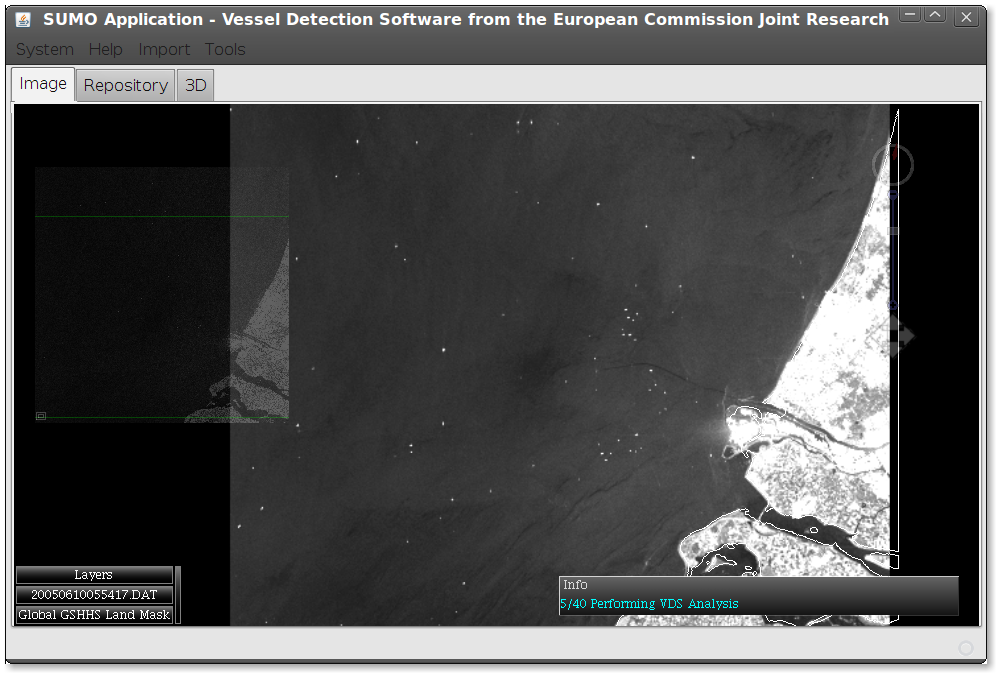
\includegraphics[scale=0.45,keepaspectratio=true]{./images/VDS3.png}
 \caption{On-going Analysis}
\end{figure}

\begin{figure}[H]
 \centering
 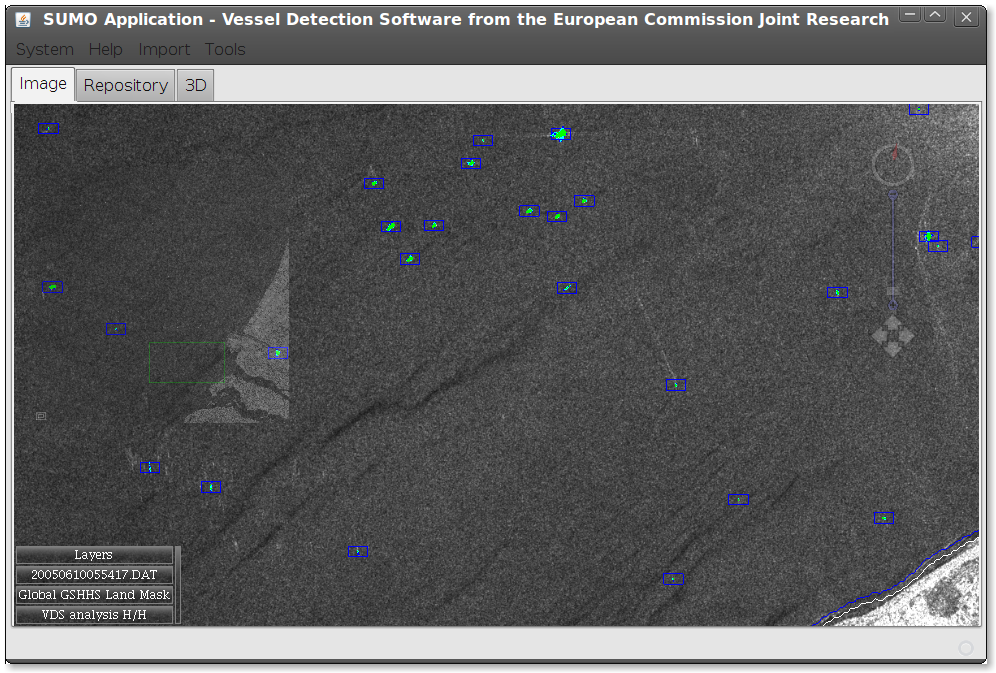
\includegraphics[scale=0.45,keepaspectratio=true]{./images/VDS4.png}
 \caption{The result of the analysis}
\end{figure}

\section{Inspecting the VDS Analysis}
In order to open the properties window of the Vector Data \textbf{Right Click} on the VDS layer.
\begin{figure}[H]
 \centering
 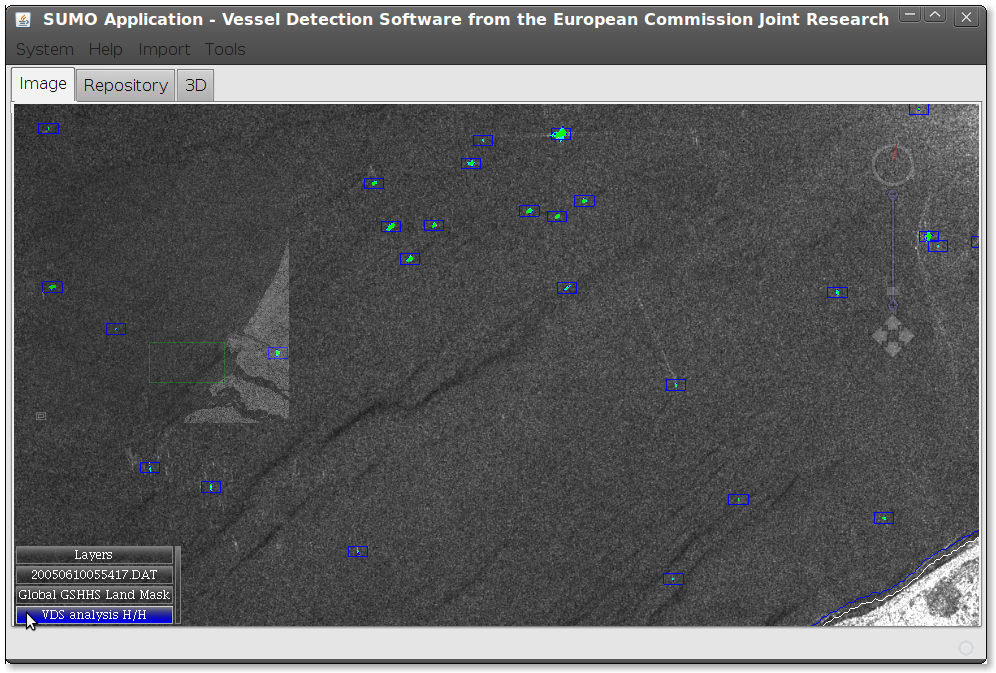
\includegraphics[scale=0.45,keepaspectratio=true]{./images/VDS5.png}
 \caption{The result of the analysis}
\end{figure}
A window will pop up with the following tabs:
\begin{enumerate}
 \item \textbf{Description}: General settings of the Layer
 \item \textbf{Style}: Let you choose some styling
 \item \textbf{Data}: The list of detected vessels with their attributes
 \item \textbf{Edit}: Let you edit the detection list (not recommended)
 \item \textbf{Info}: Show the VDS attributes when you \emph{point and click} on it.
 \item \textbf{Save}: Exporting capacities of the data (CSV, GML, XML, KML or shapefile)
\end{enumerate}
\subsection{Description}
\begin{figure}[H]
 \centering
 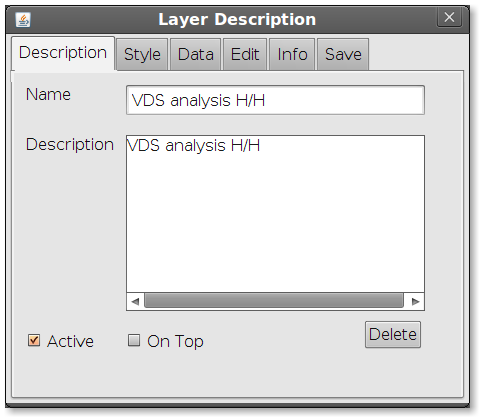
\includegraphics[scale=0.45,keepaspectratio=true]{./images/VDS6.png}
 \caption{Description Tab}
\end{figure}
\begin{itemize}
 \item \textbf{Name}: displayed name of the layer. Can be changed.
 \item \textbf{Description}: Can be changed.
 \item \textbf{Active}: will be displayed if checked.
Same as \textbf{Left Click} on the layer.
 \item \textbf{On Top}: keep this window on top of the SUMO windows.
It is useful when you need to inspect the results from the list contained in the \textbf{Data} tab.
\end{itemize}

\subsection{Style}
\begin{figure}[H]
 \centering
 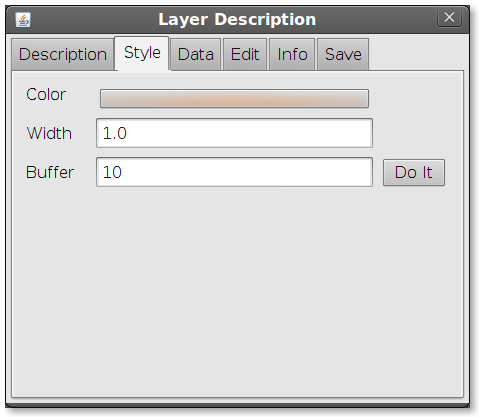
\includegraphics[scale=0.45,keepaspectratio=true]{./images/VDS7.png}
 \caption{Style tab}
\end{figure}
\begin{itemize}
 \item \textbf{Color}: let you choose the color used for the detected targets. Might be useful for comparing different analysis.
 \item \textbf{Width}: let you choose the thickness of the boxes frame that highlights the VDS.
 \item \textbf{Buffer}: let you buffer the target geometry (useless in VDS cases). Note that the geometries will be changed, there is no Undo.
\end{itemize}

\subsection{Data}
\begin{figure}[H]
 \centering
 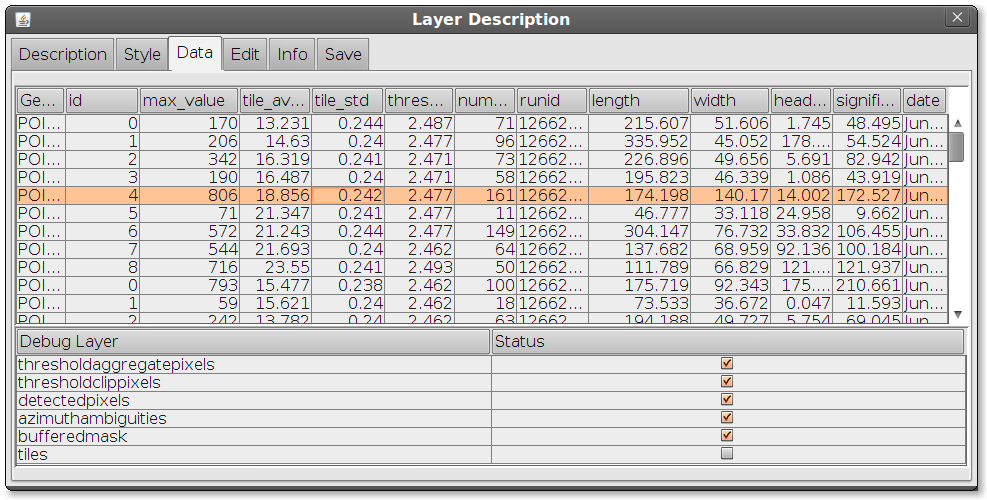
\includegraphics[scale=0.45,keepaspectratio=true]{./images/VDS8.png}
 \caption{Data tab}
\end{figure}
It contains a list of the detected targets as well as a list of extra geometry layers for in details analysis (Advanced Users only).
The list of VDS contains the following attributes:
\begin{itemize}
 \item \textbf{Geometry}: the pixel position in WKT (Well-Known Text) format. More info at \url{http://en.wikipedia.org/wiki/Well-known_text}
 \item \textbf{id}: id of the target.
 \item \textbf{max\_value}: maximum value of the target. The higher the brighter.
 \item \textbf{tile\_average}: average of the values of the tile containing the VDS.
For advanced users.
 \item \textbf{tile\_std}: standard deviation of the tile containing the VDS. For advanced users.
The higher the more noisy is the background.
 \item \textbf{threshold}: the algorithm threshold at which the detection has been made.
For advanced users.
 \item \textbf{num\_of\_pixels}: the number of pixels that have been aggregated to a single target.
The highest the bigger is the VDS.
 \item \textbf{runid}: the id of the analysis.
 \item \textbf{length} (meters): the length of the VDS.
 \item \textbf{width} (meters): the width of the target. Not much reliable and often over estimated.
 \item \textbf{heading} (degrees): direction of the target with an ambiguity of 180\textdegree.
 \item \textbf{significance}: a value computed as follow: $(max\_value-tile\_average)/tile\_std$.
The higher, the more significant is the VDS.
\end{itemize}
When you click on one of the row of the table, the app will focus automatically on the VDS.
Hitting \textbf{DEL} will remove the VDS from the table.
\emph{WARNING: there is no UNDO}.
\begin{figure}[H]
 \centering
 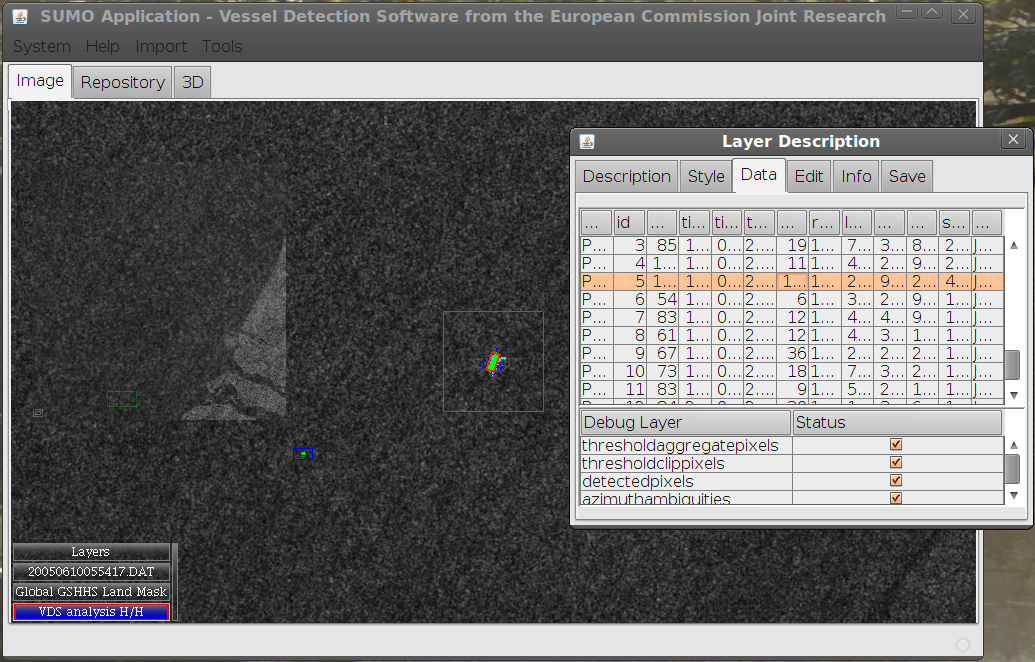
\includegraphics[scale=0.45,keepaspectratio=true]{./images/VDSInspection.png}
 \caption{Inspecting the result of the analysis}
\end{figure}

The list of extra layers are the following:
\begin{itemize}
 \item \textbf{thresholdaggregatedpixels}: showing the pixels that are over the aggregation threshold for a defined VDS
 \item \textbf{thresholdclippixels}: showing the pixels discarded from the aggregation process.
 \item \textbf{detectedpixels}: showing all the detected pixels.
 \item \textbf{azimuthambiguities}: highlights \emph{azimuth ambiguities} that are ghost VDS, not real.
 \item \textbf{bufferedmask}: showing the mask after buffering that has been used to discard the land.
 \item \textbf{tiles}: showing the tiles that have been used or the algorithm.
\end{itemize}

\subsection{Save}
\begin{figure}[H]
 \centering
 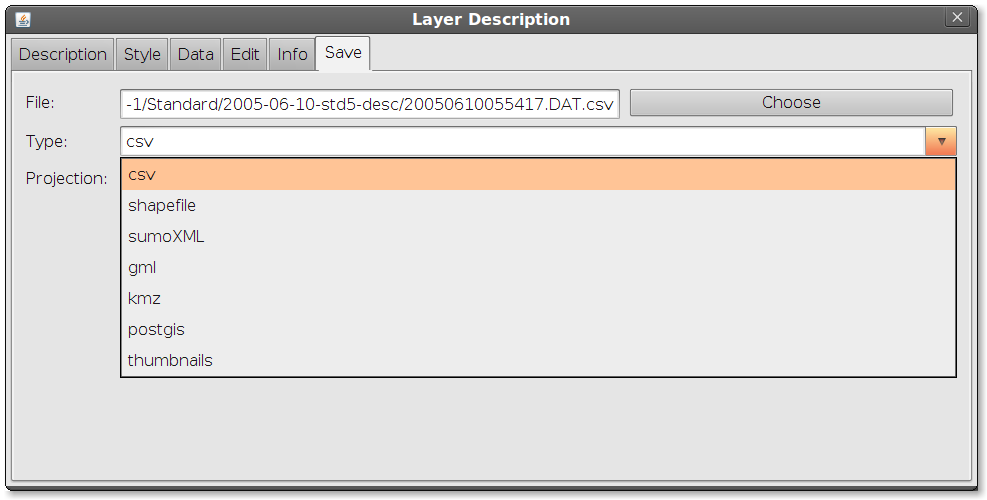
\includegraphics[scale=0.45,keepaspectratio=true]{./images/VDS9.png}
 \caption{The result of the analysis}
\end{figure}

\begin{itemize}
 \item \textbf{File}: the output file.
You can browse the file system to use.
 \item \textbf{Type}: type of the output [CSV, shapefile, SumoXML, GML (KSAT schema), kmz (Google Earth), postgis (beta), thumbnails (beta)]
 \item \textbf{Projection}: Projection of the geographic systems.
If you don't know leave as default (\textbf{EPSG:4326})
\end{itemize}

\subsection{Filtering out VDS}
In order to filter easily false alarms to keep only strong targets (usually ``big'' targets) you can use the filtering tool.
You will need access to INTERNET, more precisely to \url{http://chart.apis.google.com}.
You need to \textbf{Middle Click} to the VDS layer and a windows pops up in the view with a chart and a slider on the top.
The chart is the histogram of the significance of the targets.
On the left the less significant VDS (and probable false alarms), on the right the most significant.
Moving the sliders will filter out the less significant VDS.
\begin{figure}[H]
 \centering
 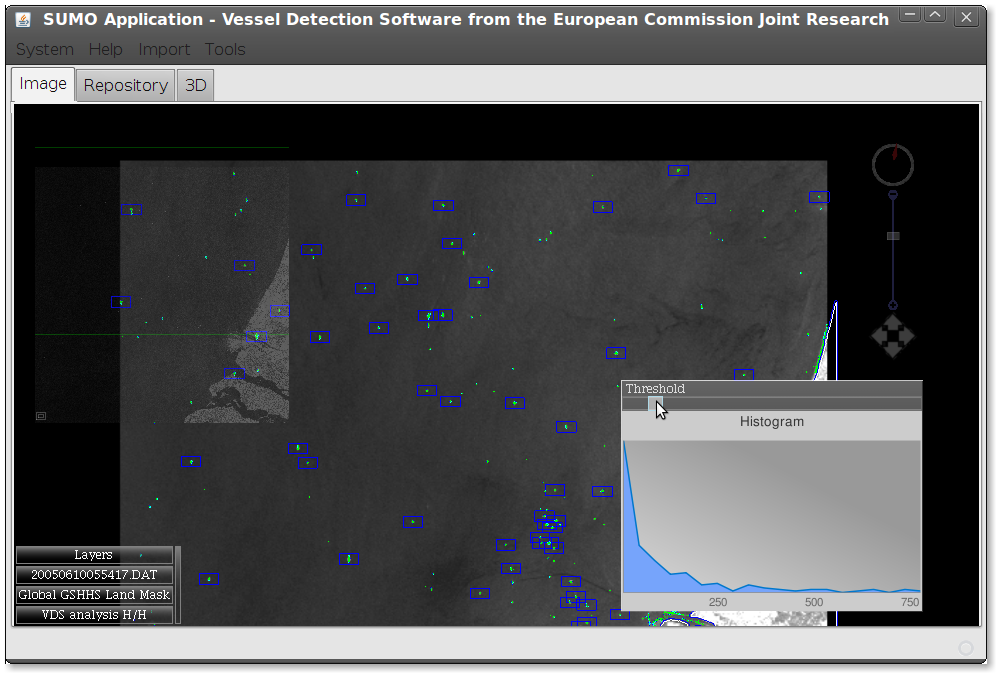
\includegraphics[scale=0.45,keepaspectratio=true]{./images/VDSThresh.png}
 \caption{The Threshold tool in action}
\end{figure}

\section{Managing the Preferences: System $>$ Preferences}
In order to change some default behaviours, it is possible to change preferences.
In the menu go to the \textbf{System $>$ Preferences} or execute the shortcut \textbf{CTRL+P}.

The list of the paramaters that can be changed are:
\begin{itemize}
 \item 
\end{itemize}

\section{Managing the Plugins: System $>$ Plugin Manager}

\end{document}          
